\section{Passivity-Based Control} \label{section:pssivity}
Initial presentation of passive-decomposition is found in D. Lee et. al 2004. \cite{passive-decomp-mechanical-coord-req}. It decomposes the overall dynamics into shape system addressing the coordination aspect, locked system representing internal dynamics wrt. the holonomic constraints and dynamic couplings between the locked and shape systems.The coupled dynamics can be canceled out without violating passivity. Thus, the coordination aspect (shape system) and the dynamics of the coordinated (locked) system can be decoupled from each other while enforcing passivity. By designing the locked and shape controls to enforce passivity  of their respective systems, the closed-loop system energetic passivity is guaranteed. A brief introduction towards passive-decomposition is given as follows. \\
Consider a group of $m$-mechanical systems such that the $i$-th agent's dynamics evolve on a configuration manifold $\Ma_i$:
	\begin{equation}
	M_i(\textbf{q}_i)\nabla^i_{\textbf{v}_i} \textbf{v}_i = \textbf{T}_i + \textbf{F}_i, \;\;\; i = 1,...,m,
\end{equation}
where the following terms are defined as follows:
\begin{itemize}
	\item $\textbf{T}_i, \textbf{F}_i\in\text{T}_{\textbf{q}_i}^*\Ma_i$ - control and environmental force covectors that exist in a cotangent manifold at point $\textbf{q}_i$
	
	\item $\textbf{v}_i \in \text{T}_i^{*}\Ma_i$ - system velocity at point $\textbf{q}_i$ in the tangent manifold
	
	\item $\nabla^i_{\textbf{v}_i}$ - this symbol represents a covariant derivative operator, the Levi-Civita connection. It provides a well defined method of differentiating vector fields along the ${\textbf{v}_i}$ direction on the tangent bundle $\text{T}\Ma_i$.
	
	\item $M_i(\textbf{q}_i)$ - inertia tensor which maps vectors from tangent space to cotangent space at point $\textbf{q}$, defined as $M:\text{T}_{\textbf{q}}\Ma \mapsto \text{T}_{\textbf{q}}^*\Ma$
\end{itemize}

Furthermore, the supply rate for the m-agent mechanical system is defined as follows.
\begin{equation}
	s_\rho(\textbf{v}_i, \textbf{T}_i) = \langle\textbf{F}_i, \dot{\textbf{q}}_i \rangle + ... + \langle\textbf{F}_m, \dot{\textbf{q}}_m \rangle \, ,
\end{equation}
where $\langle \cdot, \cdot \rangle: \text{T}_{\textbf{q}}^*\Ma \times \text{T}_{\textbf{q}}\Ma  \rightarrow \mathbb{R}$. \\
\noindent For safe and stable interaction an energetic passivity condition where $\exists d\in\mathbb{R}$ such that: 
\begin{equation}
	 \int_{0}^{t}	s_\rho(\textbf{v}_i(\tau), \textbf{T}_i(\tau))d\tau \geq -d^2, \;\forall t\geq 0
\end{equation}
Similar condition is employed to induce controller passivity.

\cite{passive-decomp-quadrotor-with-robotic-manip} 
\cite{passivity-based-formation-load}
\cite{passive-variable-impedance-compliant} 
\cite{max-wrench-min-energy} 
\cite{quadrotor-itneraction-environment} 
\cite{passivity-based-payload-minimum-swing} 
\cite{passivity-based-crop} 
\cite{payload-and-human}
\cite{door-opening} 
\cite{decoupled-aerial-manipulation} 
\cite{passivity-backstepping} 
\cite{passivity-based-physical-interaction}

\begin{figure}[H]
	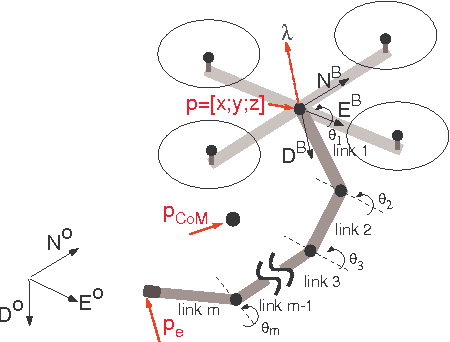
\includegraphics[width=0.9\columnwidth]{figure/aerial_manip.png}	
	\centering
	\caption{This $\text{figure}^{\cite{passive-decomp-quadrotor-with-robotic-manip}}$ represents... }
	\label{fig:aerial_manip}
\end{figure}